\begin{figure*}[!t]
\begin{minipage}[c]{1.0\columnwidth}
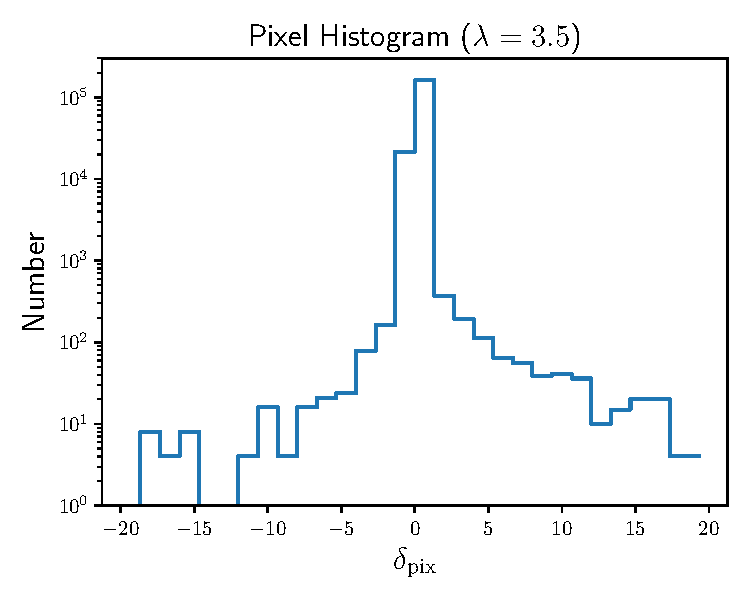
\includegraphics[width=0.95\textwidth]{pixel_histograms_halo17_NFW_lbd35.pdf}
    \includezraphics{delta-1-7-pz-wn-NFW-falsepeakproblem.pdf}
    \centering
    \small NFW: $\lambda=3.5$
\end{minipage}
\begin{minipage}[c]{1.0\columnwidth}
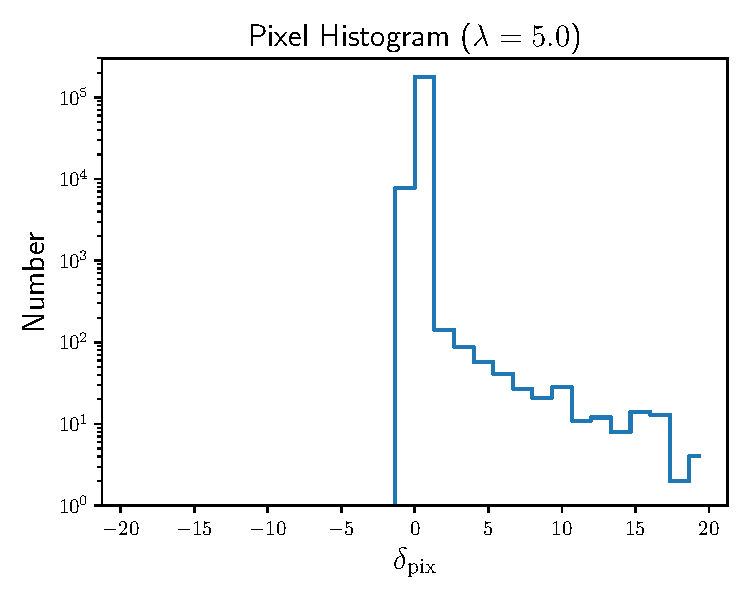
\includegraphics[width=0.95\textwidth]{pixel_histograms_halo17_NFW_lbd50.pdf}
    \includezraphics{delta-1-7-pz-wn-NFW_3-falsepeakproblem.pdf}
    \centering
    \small
    NFW: $\lambda=5.0$
\end{minipage}
\caption{The lower panels show the density maps reconstructed from the mock
    galaxy shape catalog with the NFW dictionary. The upper panels show the
    pixels' number histograms.  The penalization parameters are $\lambda=3.5$
    (left) and $\lambda=5.0$ (right).  The input halo mass is
    $M_{200}=10^{15.02} ~h^{-1}M_{\odot}$, and its redshift is $z=0.164$.  The
    vertical direction is the line of sight direction. The boxes' lower
    boundaries and upper boundaries of correspond to $z=0.01$ and $z=0.85$,
    respectively.
    } \label{fig_NFW3D}
\end{figure*}

In this subsection, we test the performance of our algorithm with the default
setup that models the matter density field with multi-scale NFW atoms. The
dictionary is constructed with three frames of different NFW scale radii in the
comoving coordinate: $0.12~h^{-1}$ Mpc, $0.24~h^{-1}$ Mpc, and $0.36~h^{-1}$
Mpc.  The truncation radii are set to four times the comoving scale radii for
the atoms in the dictionary (concentration equals four) . We note that each
frame of our dictionary fixes the scale radius in the comoving coordinates;
therefore, the NFW atoms have different angular radii in different lens
redshift bins.

We test the algorithm with different regularization parameters ($\lambda$) for
the preliminary lasso estimation, which are $3.5$, $4.0$, and $5.0$. The
corresponding regularization parameters for the final adaptive lasso
estimations are set to $\lambda_{\rm{ada}}=\lambda^{\tau+1}$.  Here, we note
that both the preliminary lasso estimation and the final adaptive lasso
estimation select the pixels with the signal-to-noise ratios (SNRs) greater
than $\lambda$ in each gradient descent iteration and estimate the density in
the selected pixels. While the final adaptive lasso estimation further enhances
the growth of the pixels with preliminary estimations greater than $\lambda$.

This paper does not go beyond the resolution limit defined by the Gaussian
smoothing kernel with a standard deviation of $1.\arcmin 5$ and the $1\arcmin$
pixel scale as discussed in Section \ref{subsec_method_smoothing} and Section
\ref{subsec_method_pixel}, respectively.  Therefore, we smooth the
reconstructed density with the same Gaussian kernel in each lens redshift
plane.

Figure \ref{fig_NFW3D} shows the $3$-D density maps reconstructed with
different penalization parameters for a halo with $M_{200}=10^{15.02}
~h^{-1}M_{\odot}$ at redshift $0.164$. Also, the pixels' histograms are shown
in Figure \ref{fig_NFW3D}. From these plots, we conclude that the adaptive
lasso algorithm sets most of the reconstructed pixels to zero and only keeps
the modes strongly related to the data. Moreover, the reconstructed density maps
do not suffer from the line of sight smearing. After the reconstruction for
each simulation, we identify the peaks on the sparse density map.

\begin{figure*}
 \centering
 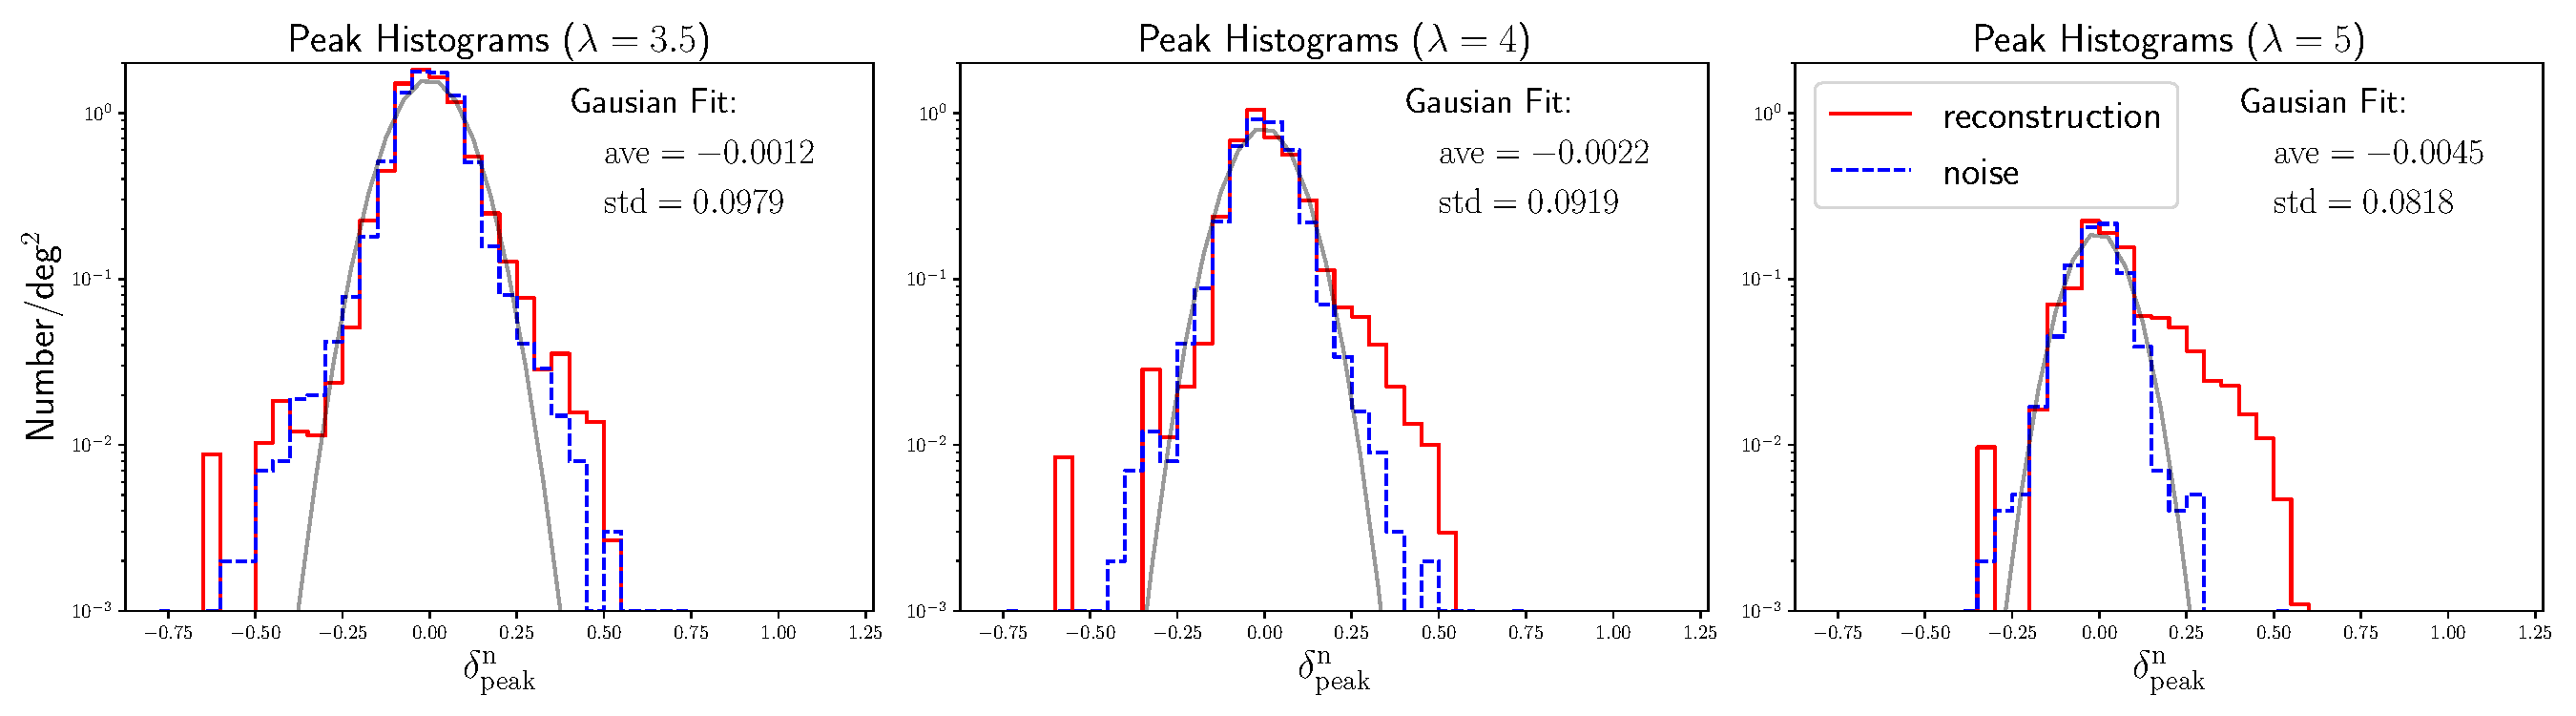
\includegraphics[width=1.0\textwidth]{peak_histograms_NFW.pdf}
 \caption{The number per square degree histograms of detected peak values from
     all of the simulations.  The solid red steps result from reconstructions
     with the NFW dictionary penalized with different regularization
     parameters: $\lambda=3.5,4.0,5.0$. The dashed blue steps are the
     corresponding results of the reconstructions from $1000$ realizations of
     pure noise catalogs. The gray lines are the best-fit Gaussian distributions
     to the noises' peak histograms.
    }\label{fig_peakHist}
\end{figure*}

Following \citet{WL-massMap-Glimpse2D-Lanusse2016}, we normalize the detected
peaks in the $l$-th ($l=1...20$) lens redshift plane to account for the peak
amplitude difference due to the difference in the norm of the lensing kernels
for different redshift bins:
\begin{equation}
\delta^{\rm{n}}_{\rm{peak}}(\vec{\theta},z_l)=\delta_{\rm{peak}}(\vec{\theta},z_l)/\mathcal{R}_{l}^{\frac{1}{2}},
\end{equation}
where the normalization matrix is defined as
\begin{equation}
\mathcal{R}_{l}=\sum_s K^2(z_l,z_s).
\end{equation}
The solid steps in Figure \ref{fig_peakHist} show the histograms of the
normalized peaks with different penalization parameters. Also, we simulate
$1000$ realizations of pure noise catalogs and perform the reconstructions on
these noise catalogs to study the noise properties. The dashed steps in Figure
\ref{fig_peakHist} show the histograms of normalized peaks detected from the
pure noise catalogs. The solid lines in Figure \ref{fig_peakHist} show the
best-fit Gaussian distributions to the noise peaks' histograms.

Figure \ref{fig_peakHist} tells that the densities of peaks (including both
true and false peaks) are suppressed as the penalization parameter $\lambda$
increases. Moreover, we find the standard deviation of noise peaks slightly
decreases as $\lambda$ increases. As a result, for a higher detection threshold
($\lambda=5.0$), we find a clearer peak number excess for mass maps
reconstructed from mock catalogs comparing with the noise peak histogram .

The $2$-D histogram, stacked from all of the simulations, for the offsets of
the detected peak positions from the input halos' positions is shown in the
left panel of Figure \ref{fig_detoffsets}. We see a clustering of peaks close
to the input halo's position on the stacked position histogram.  For each stamp
simulation, we find the positive peak closest to the input position (in the
pixel unit). If the closest peak lay inside the region denoted with the dashed
box in the left panel of Figure \ref{fig_detoffsets}, we take it as a true peak
detection of the input halo. Other identified peaks, which include both positive
and negative peaks, are taken as false detections.

\begin{figure*}
 \centering
 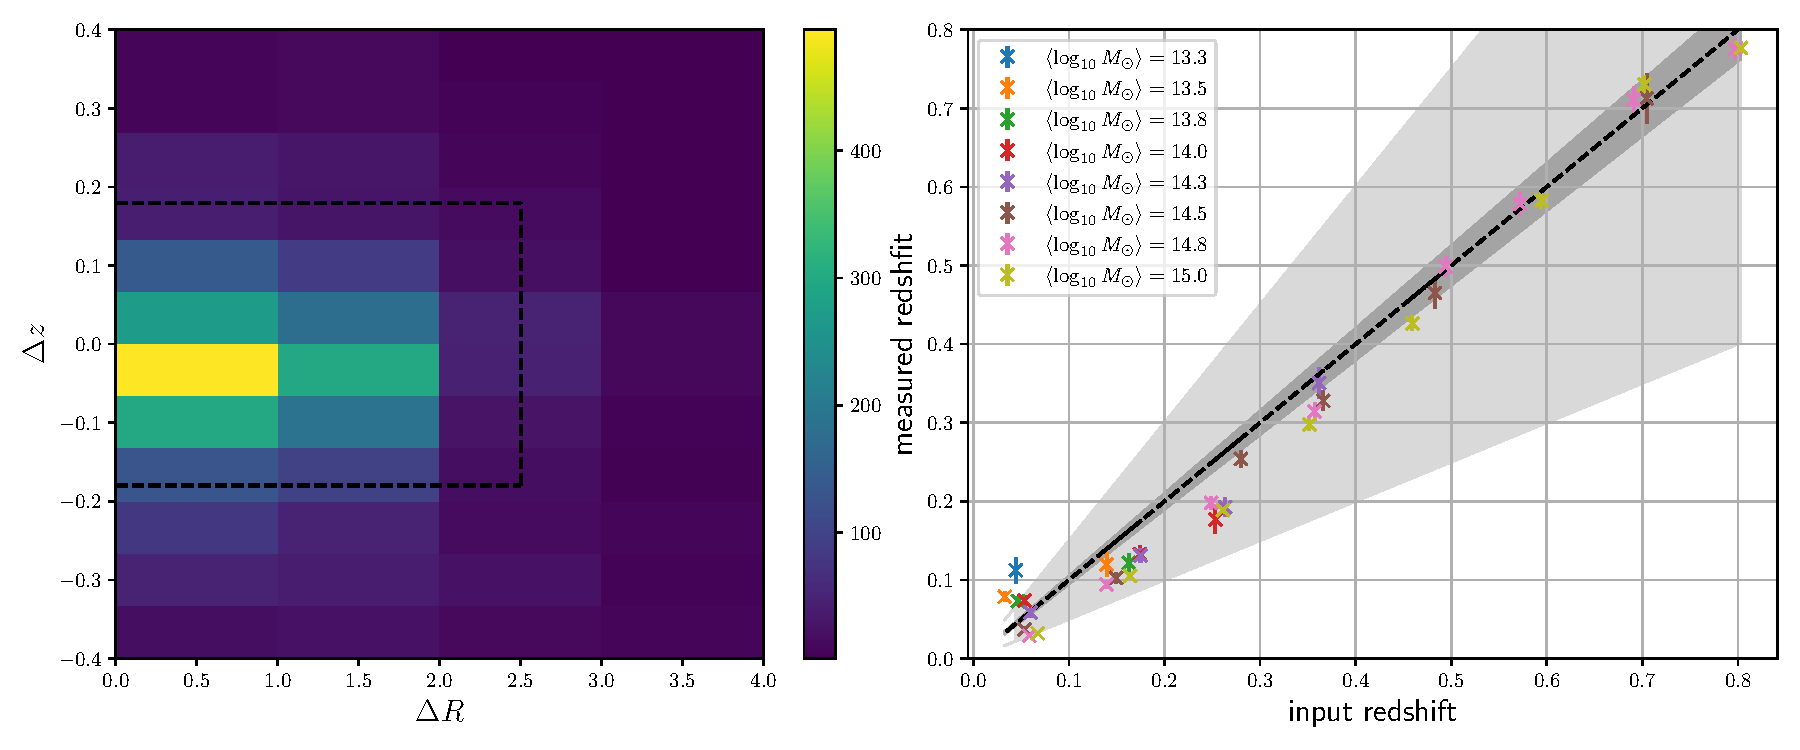
\includegraphics[width=1.0\textwidth]{peak_scatters_NFW_lbd35.pdf}
 \caption{The left panel shows the stacked $2$-D distribution of the deviations
     of detected peak positions from the centers of the corresponding input
     halos. The $x$-axis is for the deviated distance in the transverse plane,
     and the $y$-axis is for the deviation of the redshift. For each
     simulation, the positive peak inside the dashed black box with the minimal
     offset (in the pixel unit) from the input halo's position is taken as a
     true detection. The right panel focuses on the deviation of detected peaks
     in the line of sight direction. The $x$-axis is the input halo redshifts,
     and the $y$-axis is the redshift of the detected peak. The `$\cross$'
     denotes the average redshift of detected peaks for each halo over
     different noise realizations, and the error-bars are the uncertainties of
     the average redshifts. The deep gray area is for the relative redshift
     bias less than $0.05$, and the light gray area is for the relative
     redshift bias less than $0.5$. These results in this figure are based on
     the NFW dictionary with $\lambda=3.5$.
     } \label{fig_detoffsets}
\end{figure*}

The right panel of Figure \ref{fig_detoffsets} shows the average redshift of
true detections for each halo. The estimated redshifts are lower than the true
redshifts by about $0.03$ for halos in the low-redshift range ($z\leq
0.4$).  For halos at $0.4<z\leq 0.85$, the relative redshift bias is below
$0.5\%$.

With the intent to suppress false detections, we select peaks with values
greater than an ad-hoc threshold as candidates of galaxy clusters following
\citet{HSC1-massMap-cluster}.  The threshold is set to a few times the standard
deviation of the noise peaks. We use different detection thresholds
($1.5\sigma$ and $3.0\sigma$) to detect galaxy clusters from the mass maps
reconstructed with $\lambda=3.5,4.0,5.0$. The left and middle columns of Figure
\ref{fig_detFalsRateNFW} show the detection rates for halos in the (mass,
redshift) planes with detection thresholds set to $1.5\sigma$ and $3.0\sigma$
of the noise peaks' distributions, respectively.  The right column of Figure
\ref{fig_detFalsRateNFW} shows the corresponding numbers of false detections
per square degree as functions of detection thresholds. The first, second, and
third rows of Figure \ref{fig_detFalsRateNFW} correspond to the
$lambda=3.5,4.0,5.0$, respectively.

Figure \ref{fig_detFalsRateNFW} tells that the false peak density is suppressed
as the detection threshold increases. Also, the detection rate of halo
significantly decreases. We decide to set the detection threshold to
$1.5\sigma$ and set the penalization parameter $\lambda$ to $5.0$ since such a
setup suppresses the false detection to $0.022$ while keeping a good halo
detection rate. In summary, The algorithm is able to detect halo with minimal
mass limits of $10^{14.0} M_{\odot}/h$, $10^{14.7} M_{\odot}/h$, $10^{15.0}
M_{\odot}/h$ for the low ($z<0.3$), median ($0.3\leq z< 0.6$) and high
($0.6\leq z< 0.85$) redshifts, respectively.

\begin{figure*}
 \centering
 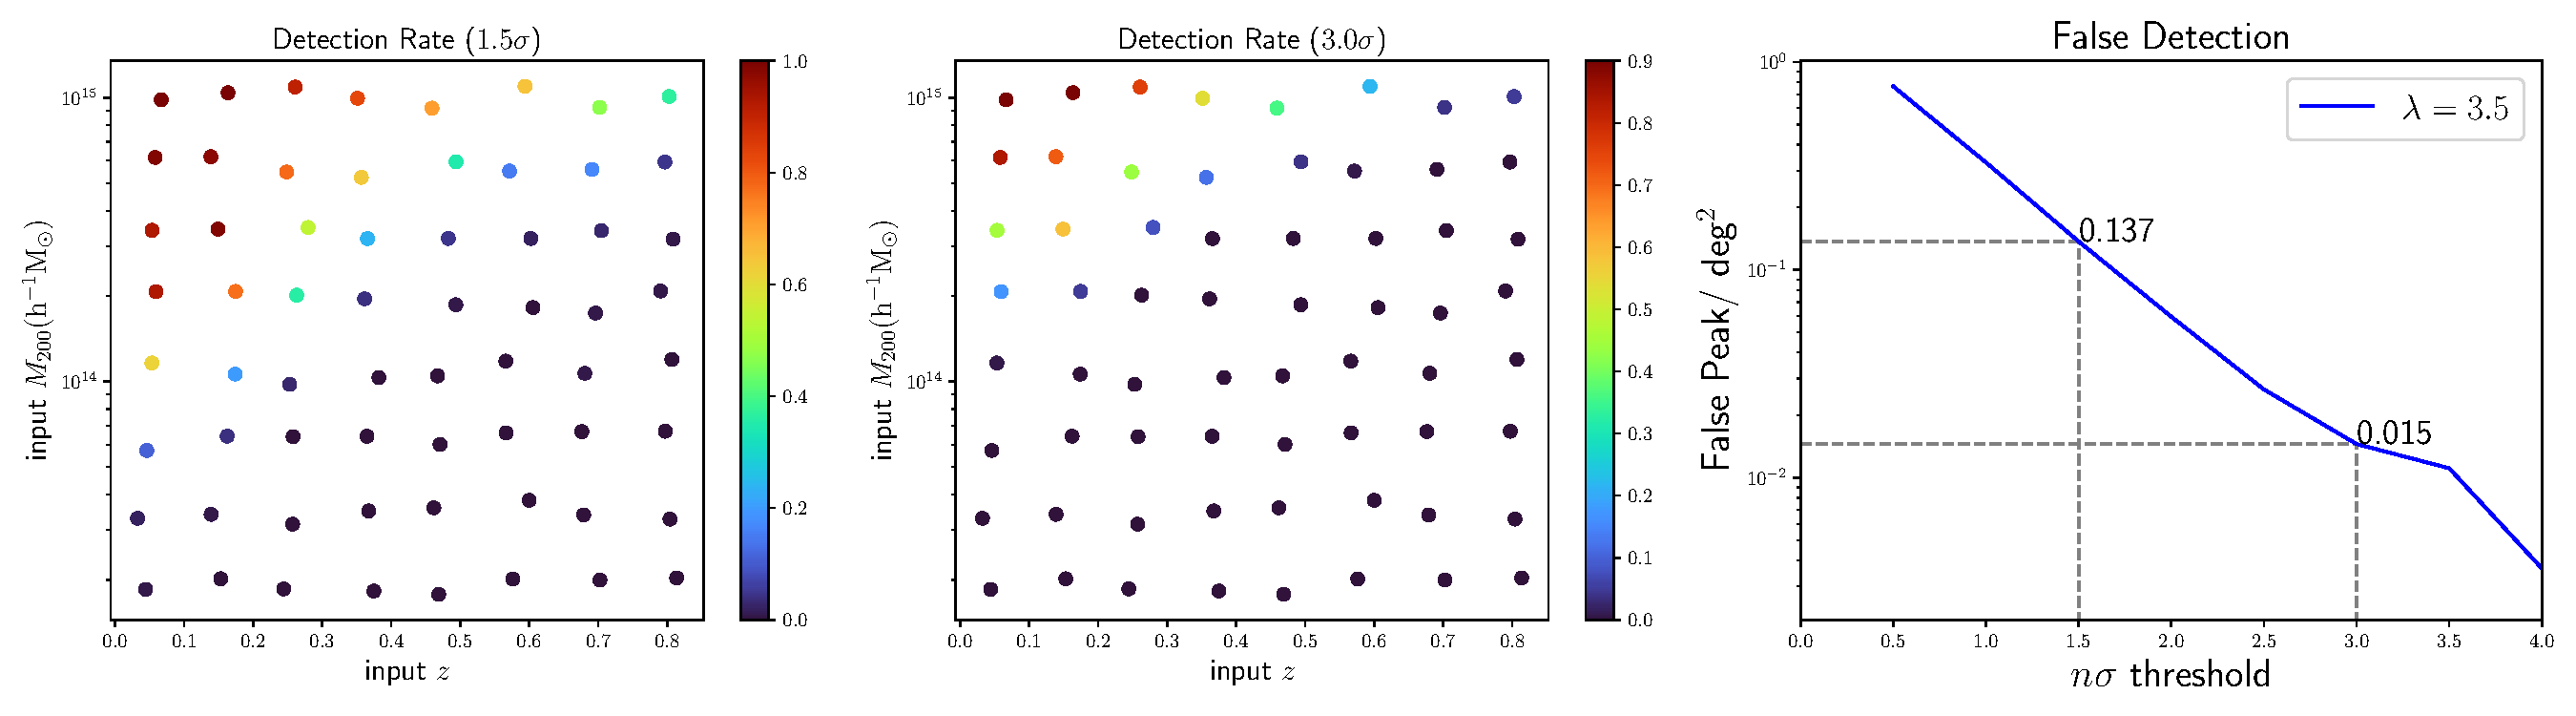
\includegraphics[width=1.0\textwidth]{detfalse_threshold_NFW_lbd35.pdf}
 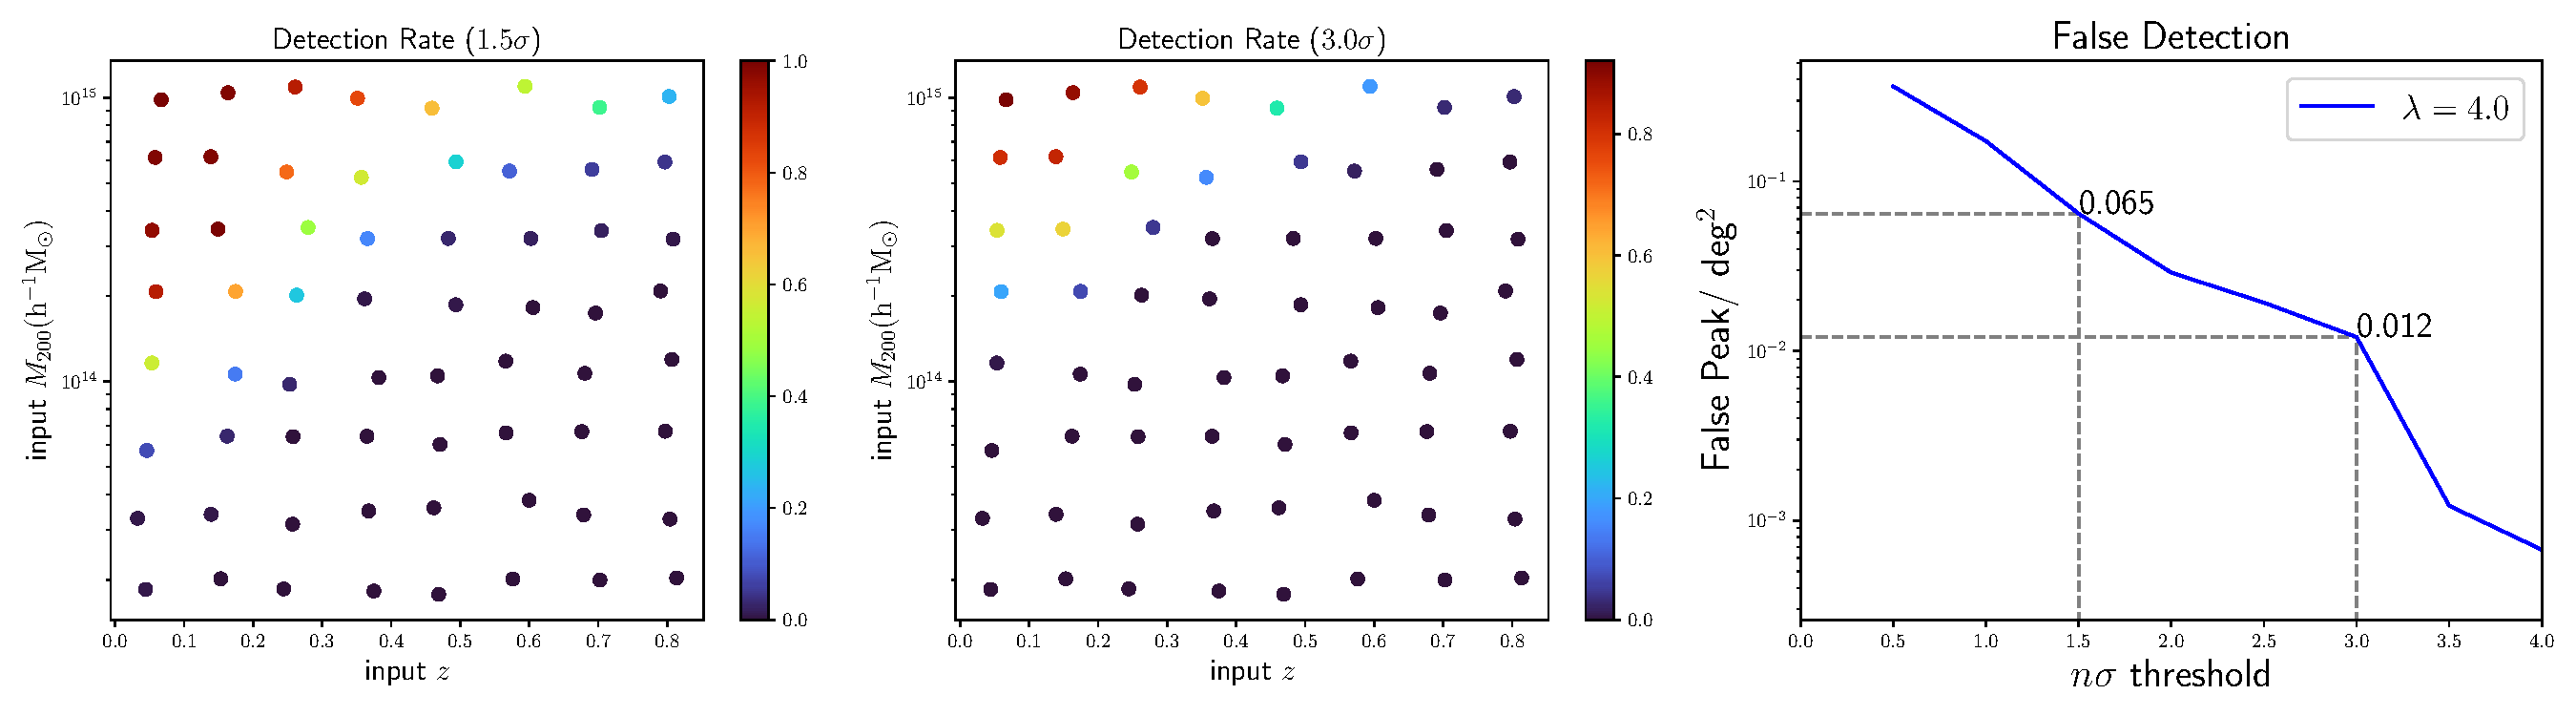
\includegraphics[width=1.0\textwidth]{detfalse_threshold_NFW_lbd40.pdf}
 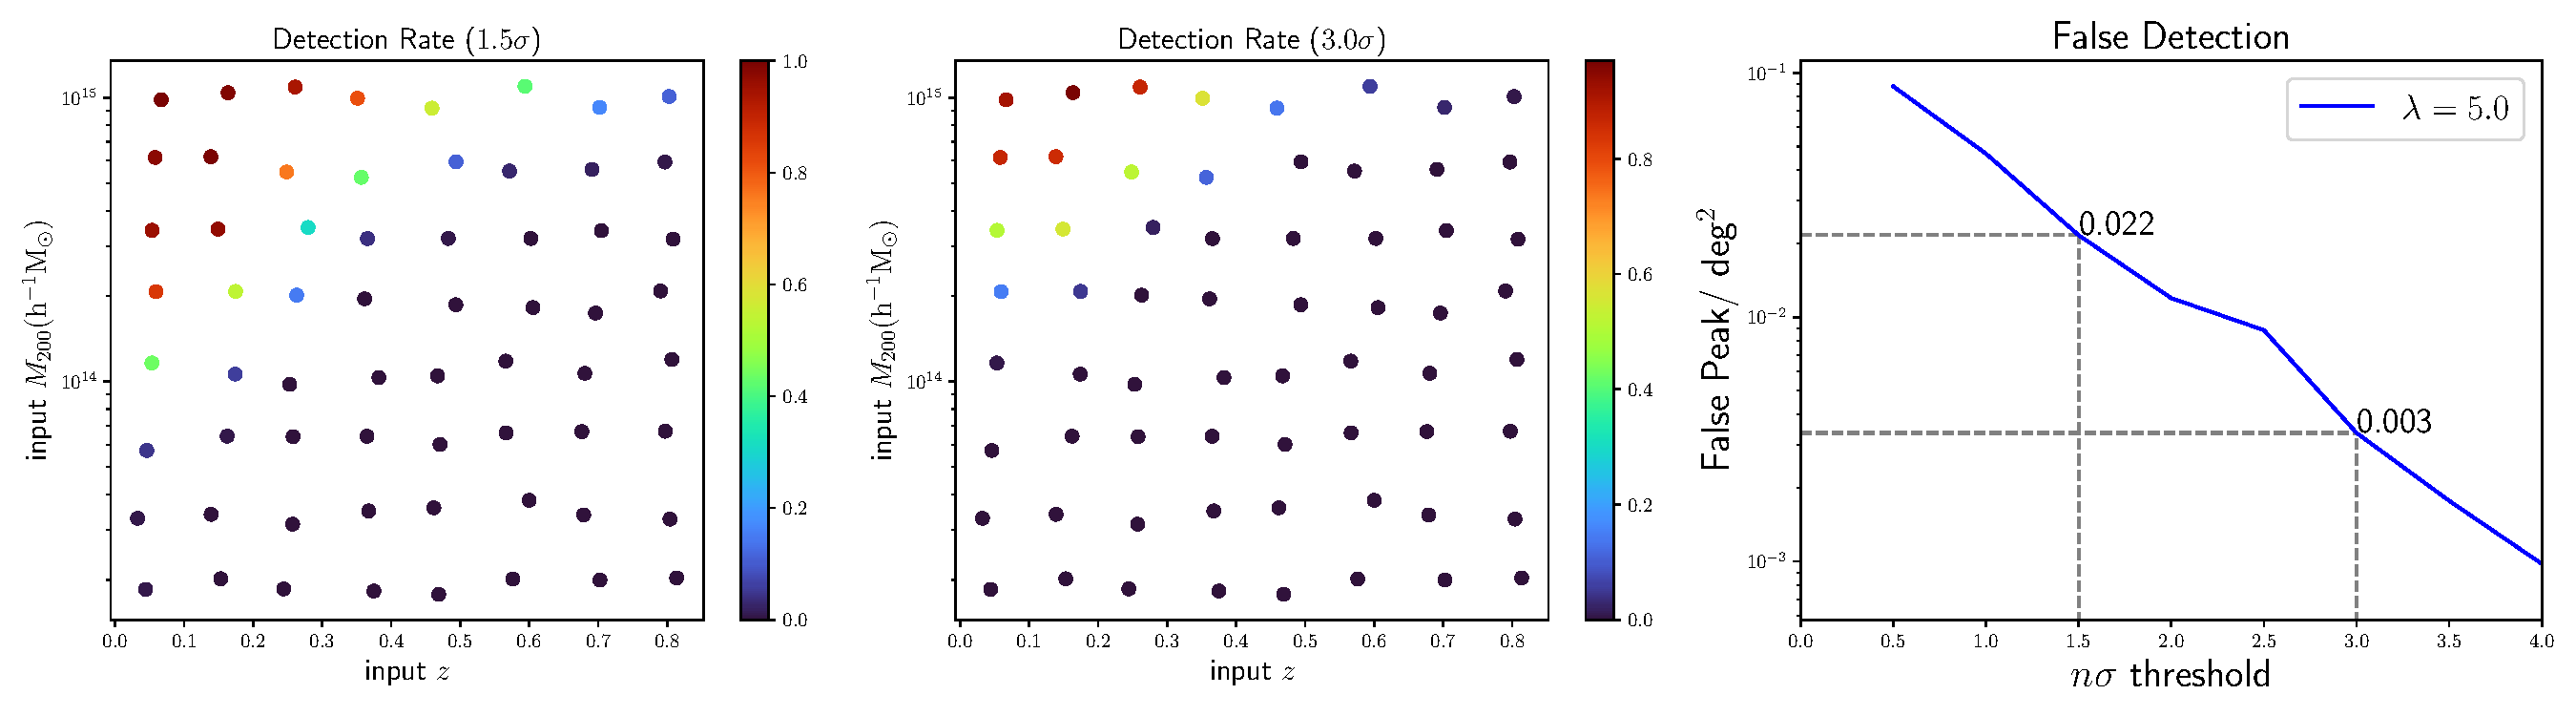
\includegraphics[width=1.0\textwidth]{detfalse_threshold_NFW_lbd50.pdf}
 \caption{The detection rates and false peak densities for different
     penalization parameters and detection thresholds. The first, second, and
     third rows correspond to the results with $\lambda=3.5,4.0,5.0$,
     respectively. The left and middle columns are the halo detection rates for
     detection thresholds equal $1.5\sigma$ and $3.0\sigma$, respectively. The
     right column shows the density of false peaks as a function of detection
     threshold.
    } \label{fig_detFalsRateNFW}
\end{figure*}

